% p21-f-dagger-completes-the-following-diagram.tex
%
% Source:   Carl A. Gunter and Dana S. Scott, "Semantic Domains".
%           ScottDomains/papers/Gunter Scott 1990.pdf
% Physical page: 21          Printed page: 20
% Section:  4.4 Sums and lifts.
% Unnamed in the paper (no figure number). Introduced by:
%   "Given cpo's D and E and continuous function f : D -> E, there is a unique
%    strict continuous function f-dagger which completes the following
%    diagram:"
%
% Content: the universal property of the lift, the same triangle shape as the
% smash-product diagram on page 19. Vertices 3, arrows 3 (2 solid, 1 dashed).
%
% Geometry measured from a 300 dpi render of the region and divided by
% 118.11 px/cm.
%
\documentclass[border=6pt]{standalone}
\usepackage{tikz}
\begin{document}
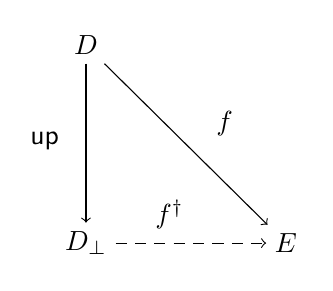
\begin{tikzpicture}[
  x=1cm, y=1cm,
  every node/.style={inner sep=1pt},
  open/.style={circle, draw, fill=white, minimum size=4pt, inner sep=0pt},
  solid/.style={circle, draw, fill=black, minimum size=5pt, inner sep=0pt},
  edge/.style={draw, line width=0.4pt},
  % added for the commutative diagrams: object nodes, and the paper's two
  % arrow kinds -- solid for a named map, dashed for the unique completing map
  obj/.style={inner sep=3pt},
  arrow/.style={draw, line width=0.4pt, ->},
  darrow/.style={draw, line width=0.4pt, ->, dash pattern=on 4pt off 3pt}]

  % vertices
  \node[obj] (d)    at (0.00,2.51) {$D$};
  \node[obj] (dbot) at (0.00,0.00) {$D_{\bot}$};
  \node[obj] (e)    at (2.54,0.00) {$E$};

  % arrows
  \draw[arrow]  (d)    -- (dbot);
  \draw[arrow]  (d)    -- (e);
  \draw[darrow] (dbot) -- (e);

  % labels printed inside the picture
  \node[anchor=east] at (-0.30,1.30) {\textsf{up}};
  \node at (1.76,1.52) {$f$};
  \node at (1.06,0.36) {$f^{\dagger}$};
\end{tikzpicture}
\end{document}
